% Paper draft for FPGA 2015
\documentclass{acm_proc_article-sp}
\usepackage{graphicx}
\usepackage{multirow}
\usepackage[caption=true,font=footnotesize]{subfig}
\usepackage{dblfloatfix}
\usepackage{algorithmic}
\usepackage{algorithm}
\usepackage{xspace}
\usepackage{url}
\usepackage{bm}
%\renewcommand{\topfraction}{0.5}
%\renewcommand{\dbltopfraction}{0.5}

\renewcommand\floatpagefraction{.9}
\renewcommand\topfraction{.9}
\renewcommand\bottomfraction{.9}
\renewcommand\dbltopfraction{.9}
\renewcommand\textfraction{.1}   
\setcounter{totalnumber}{50}
\setcounter{topnumber}{50}
\setcounter{bottomnumber}{50}

\newcommand{\eqnref}[1]{(\ref{#1})}
\newcommand{\figref}[1]{Figure~\ref{#1}}
\newcommand{\algref}[1]{Algorithm~\ref{#1}}
\newcommand{\secref}[1]{Section~\ref{#1}}
\newcommand{\tabref}[1]{Table~\ref{#1}}
\newcommand{\autoesl}{AutoESL\xspace}
\newcommand{\tabincell}[2]{\begin{tabular}{@{}#1@{}}#2\end{tabular}}

\usepackage{etoolbox}
\makeatletter
\patchcmd{\maketitle}{\@copyrightspace}{}{}{}
\makeatother
\graphicspath{{./figures/}}

\begin{document}

\title{Automatic Soft CGRA Overlay Customization for High-Productivity 
Nested Loop Acceleration on FPGAs}

\numberofauthors{1}
 \author{
 \alignauthor
 Cheng Liu, Hayden Kwok-Hay So\\
        \affaddr{Department of Electrical and Electronic Engineering, 
        The University of Hong Kong}\\
        \email{\{liucheng, hso\}@eee.hku.hk}
 }
\maketitle

% A category with the (minimum) three required fields
%\category{H.4}{Information Systems Applications}{Miscellaneous}
% A category including the fourth, optional field follows...
%\category{D.2.3}{Hardware Engineering}{Metrics}[complexity measures, performance measures]
%\terms{Theory}
%\keywords{High Level Synthesis, Soft Coarse Grain Reconfigurable Array, Design Productivity, High Frequency FPGA Design}

\section{Introudction} \label{introduction}
Compiling high level compute intensive kernels 
to FPGAs via an abstract overlay architecture 
has been demonstrated to be an effective way to 
improve designers' productivity. 
However, achieving the desired performance and 
overhead constraints requires exploration in a 
complex design space involving multiple 
architectural parameters and counteracts 
the benefit of utilizing an overlay 
as a productivity enhancer.

In this work, a soft CGRA (SCGRA) which provides unique 
opportunity to improve the power-performance of the 
resulting accelerators is used an FPGA overlay. 
With the observation that the loop unrolling factor and SCGRA size 
typically have monotonic 
impact on the loop compute time and the loop performance 
benefit degrades with the increase of the two design parameters, 
we took a marginal performance revenue metric to prune the 
design space to a small feasible design space (FDS) and then 
performed an intensive customization on the 
FDS by using analytical models of various design metrics 
such as power and overhead.

\section{Proposed Customization Framework} \label{sec:dse-framework}
\figref{fig:customization-framework} illustrates the proposed customization 
framework for nested loop acceleration using an SCGRA overlay. Centering the 
SCGRA size and loop unrolling factor, the revenue aware (RA) 
design space exploration (DSE) algorithm is applied to acquire a feasible 
sub design space. By taking advantage 
of the regularity of the SCGRA overlay, the design metrics such as power and energy 
of the FDS can be explored effectively and customization 
for various design goals can be obtained. Afterwards, the customized 
accelerator and communication interface can be generated. Then both the 
software running on host CPU and the generated accelerator can be compiled to  
the CPU-FPGA system rapidly. 
 
\section{Experiments \& results}
We take four applications including Matrix Multiplication (MM), 
FIR, Kmean(KM) and Sobel Edge Detector (SE) as our benchmark. In order to 
evaluate the quality and efficiency of the proposed design framework, we
have the benchmark implemented using both the proposed RA 
DSE and an exhaustive search (ES) based DSE. As shown in 
\figref{fig:DSE-Time} and \figref{fig:DSE2}, when compared to the ES based DSE,
the proposed customization framework reduces run time by 2 orders 
of magnitude on average while producing similar energy-performance 
Pareto-optimal curve and the same customized architecture 
that achieves minimum energy consumption. 
\begin{figure}[tbh]
\center{\includegraphics[width=0.65\linewidth]{customization-framework}}
\caption{The proposed customization framework}
\label{fig:customization-framework}
\end{figure}

\begin{figure}[tbh]
    \centering
    \includegraphics[width=0.32\textwidth]{DSE-Time}
    \caption{RA DSE Vs. ES DSE}
    \label{fig:DSE-Time}
\end{figure}

\begin{figure}[tbh]
    \centering
	\subfloat[MM]{%
		\includegraphics[width=0.2\textwidth]{mm-energy-perf}
	}
	\subfloat[FIR]{%
		\includegraphics[width=0.2\textwidth]{fir-energy-perf}
	}
    \hfill
	\subfloat[SE]{%
		\includegraphics[width=0.2\textwidth]{se-energy-perf}
	}
	\subfloat[KM]{%
		\includegraphics[width=0.2\textwidth]{km-energy-perf}
	}
    \caption{Performance-energy Pareto-optimal curve}
	\label{fig:DSE2}
\end{figure}


\end{document}

